\section{Результати алгоритму Б-К та згорткових нейромереж}

В даній роботі добре проявив себе метод Б-К (рис. \ref{fig:bk_examples}),
а саме програмна бібліотека PyMaxflow,
що базується на бібліотеці maxflow, автором якої є сам Володимир Колмогоров.

\begin{figure}[H]
    \centering

    \subfloat[\cite{krygin_geometry}]{
        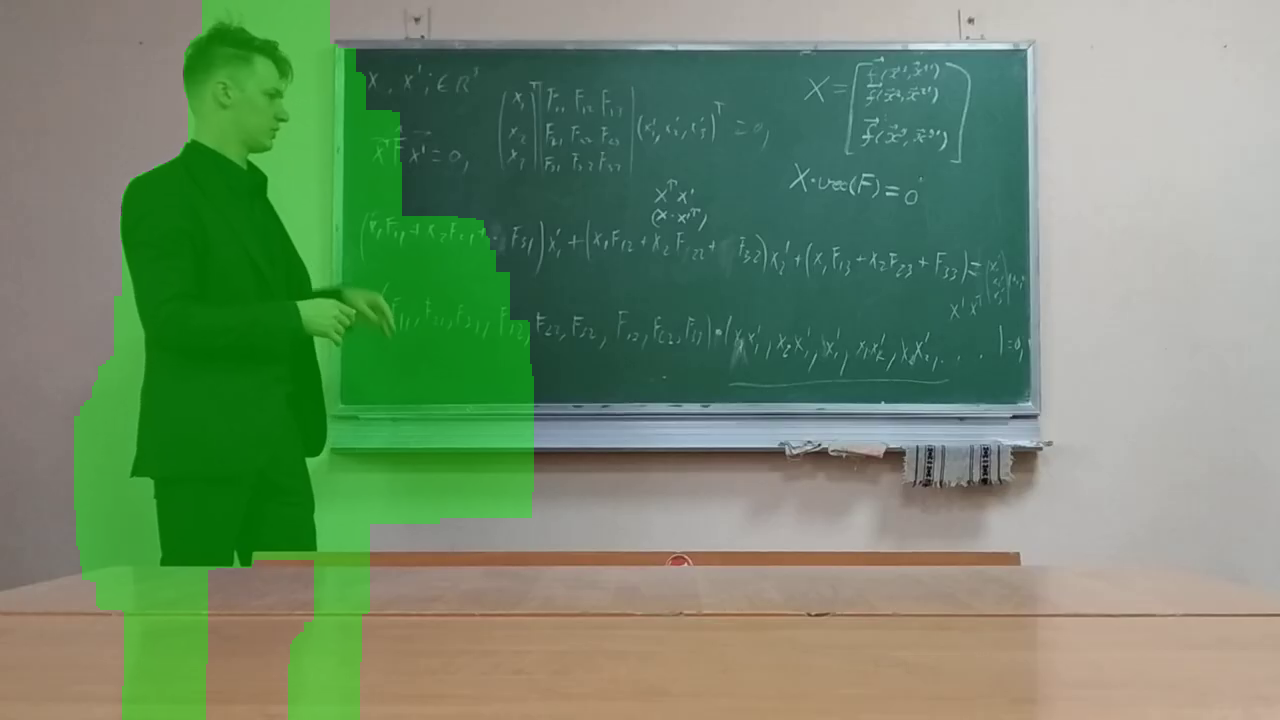
\includegraphics[width=0.35\textwidth]{images/krygin_geometry_bk_17300}
    }
    \subfloat[\cite{algebra_geometry}]{
        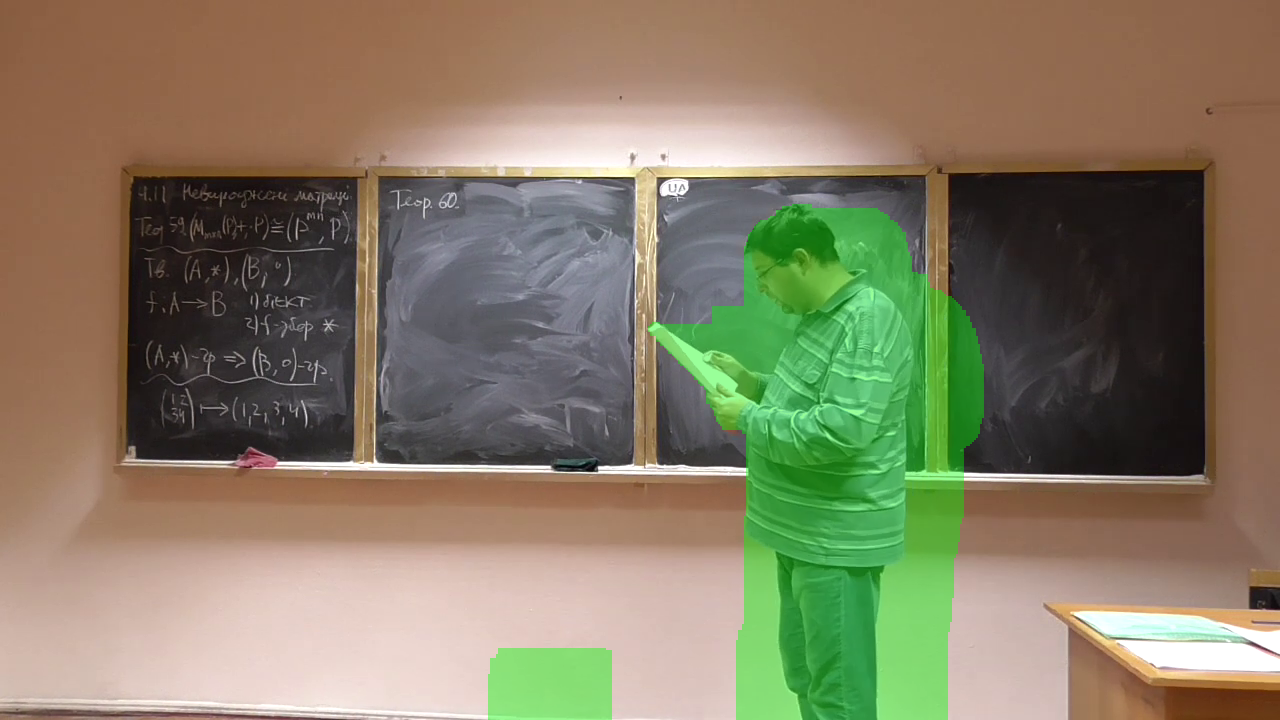
\includegraphics[width=0.35\textwidth]{images/algebra_geometry_bk_9650}
    }\\
    \subfloat[\cite{yakovlev_numbers_theory_video}]{
        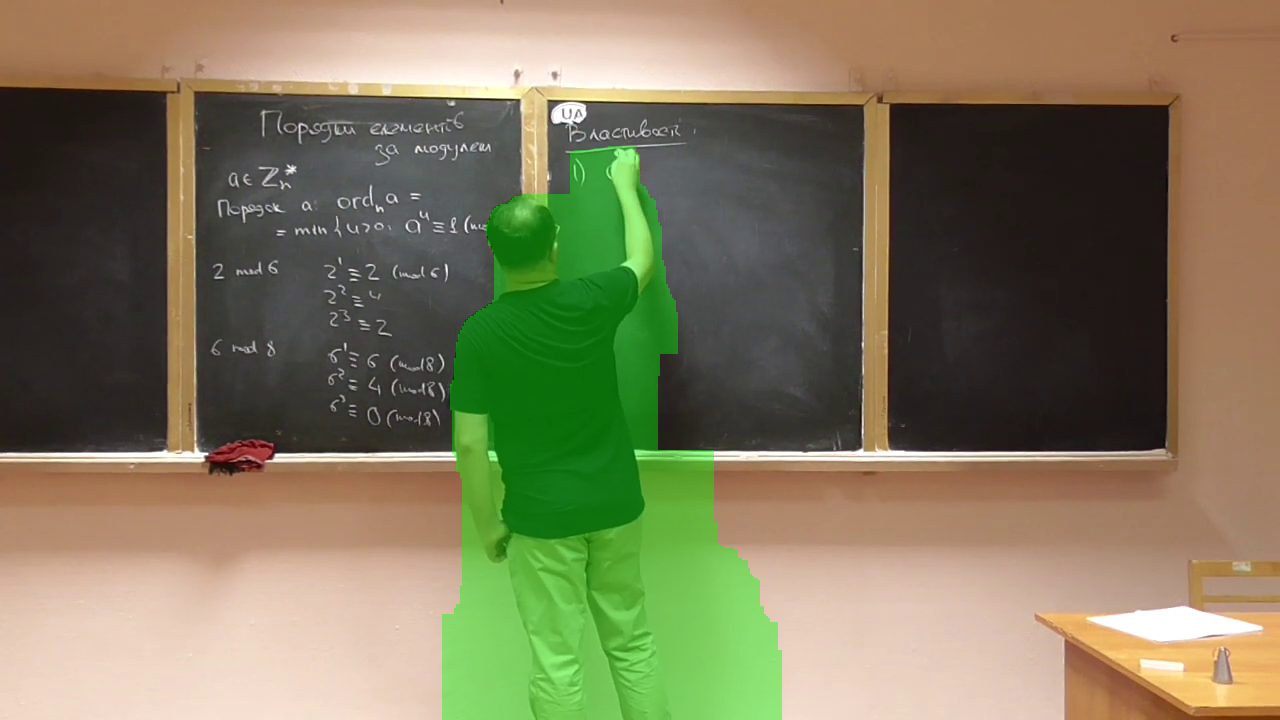
\includegraphics[width=0.35\textwidth]{images/yakovlev2_bk_6500}
    }
    \subfloat[\cite{dorohovtsev_wiener_video}]{
        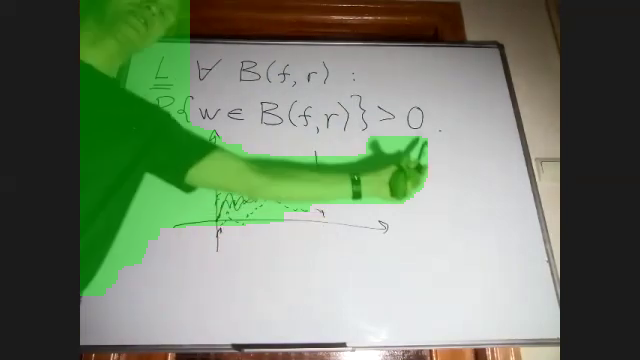
\includegraphics[width=0.35\textwidth]{images/dorohovtsev2_bk_10650}
    }
    \caption{Приклад роботи алгоритму Б-К для отримання маски рухомих об'єктів
        \label{fig:bk_examples}
    }
\end{figure}

Переваги алгоритму Б-К:
\begin{enumerate}
    \item алгоритм Б-К досить швидко будує мінімальний розріз. В середньому
          потрібно 0.2 секунди для кадру розміром $330 \times 640$.
    \item даний метод не потребує ніякої передобробки, тобто не потрібно навчати
          як нейронну нейромережу.
\end{enumerate}

Недоліки алгоритму Б-К:
\begin{enumerate}
    \item оскільки даний метод локалізує рух на кадрах відео,
          при русі камери практично все, що в кадрі, стає рухомим об'єктом
          (рис.\ref{fig:bk_bad_mask}).
          Частково дана проблема вирішена на другому кроці алгоритму створення панорами
          (алг. \ref{al:panorama_creating_algorithm});
    \item якщо викладач практично не рухається впродовж довгого часу, відповідно не потрапляє
          на маску рухомих об'єктів, він може потрапити на панорамний слайд.
\end{enumerate}

\begin{figure}[H]
    \centering

    \subfloat[]{
        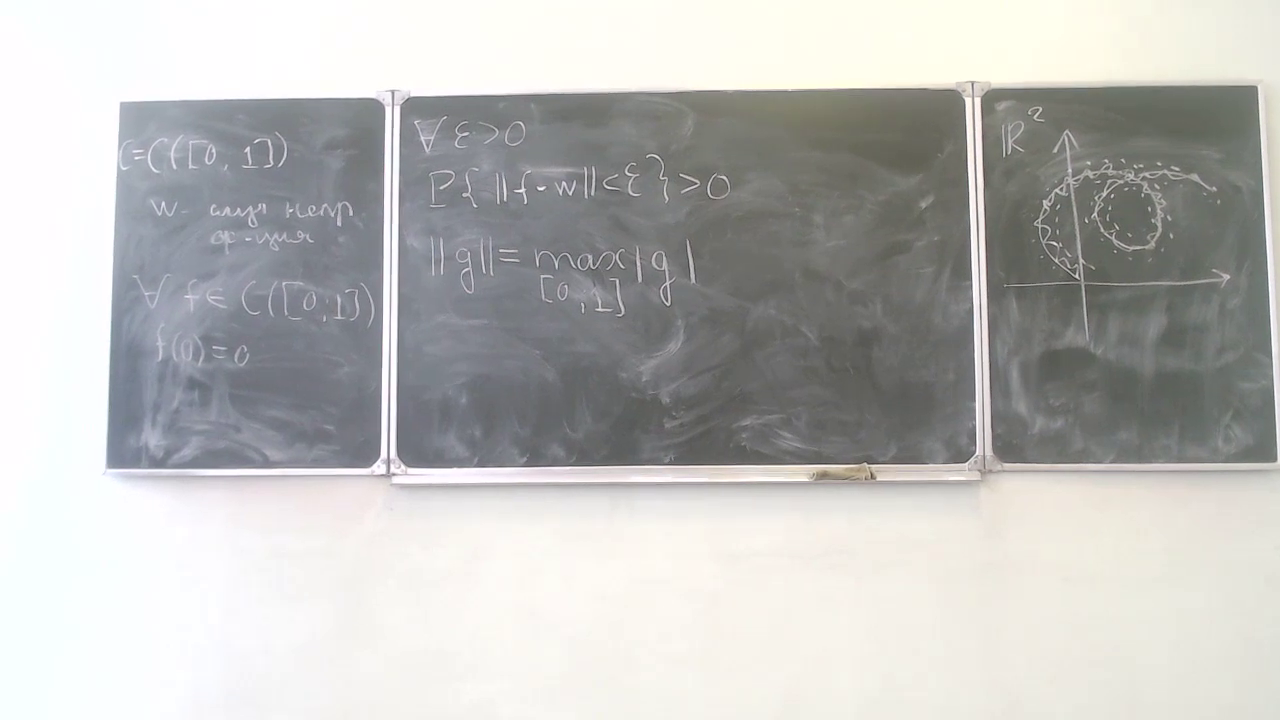
\includegraphics[width=0.35\textwidth]{images/bad_prev_dorohovtsev_bk_5790}
    }
    \subfloat[]{
        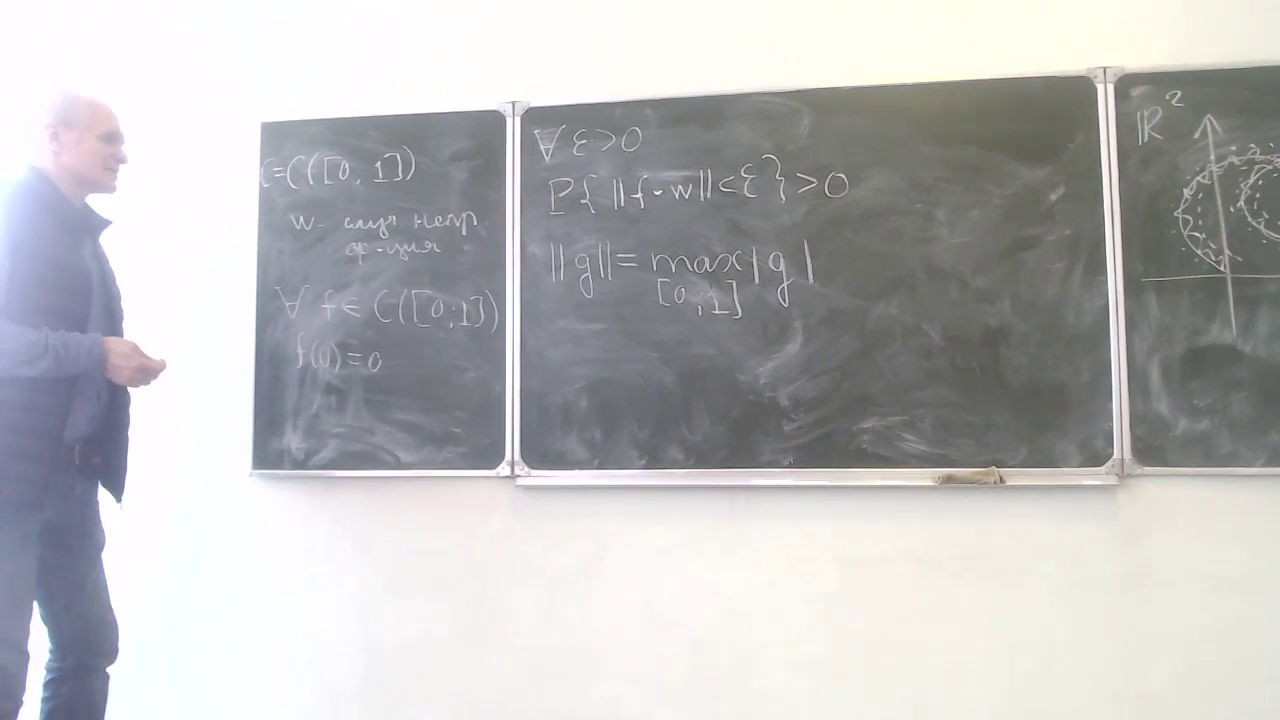
\includegraphics[width=0.35\textwidth]{images/bad_next_dorohovtsev_bk_5840}
    } \\
    \subfloat[]{
        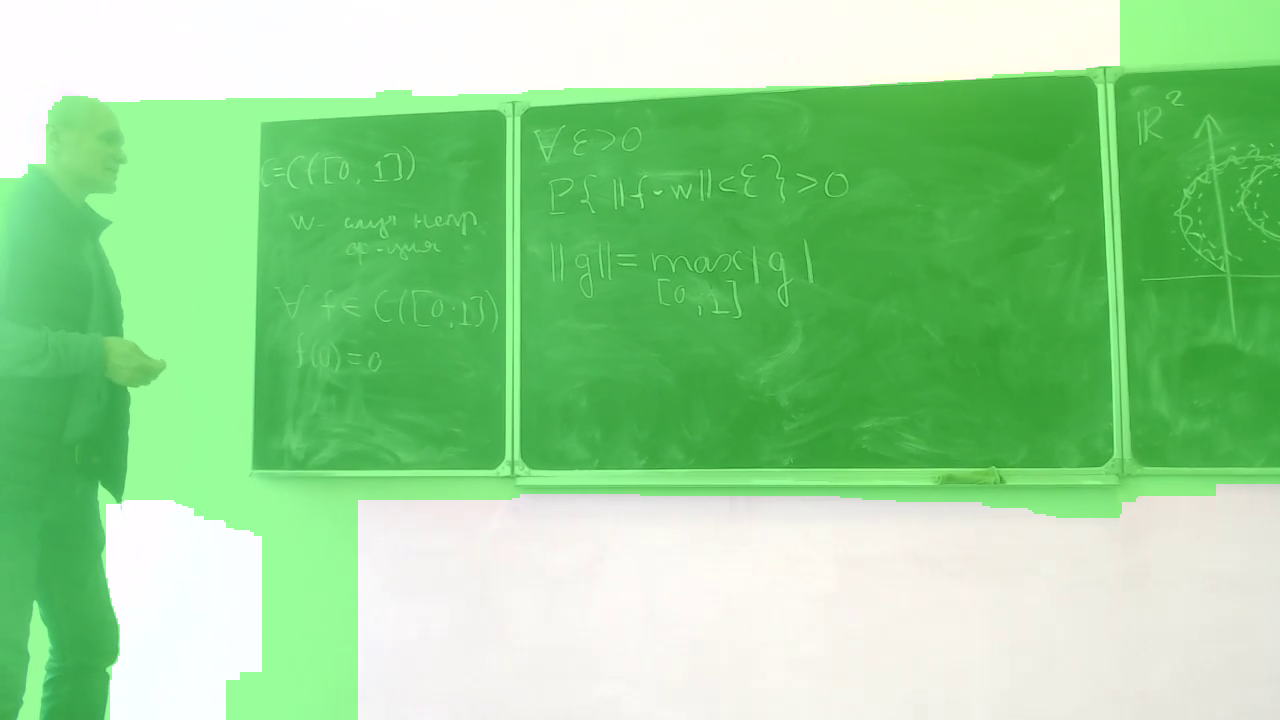
\includegraphics[width=0.35\textwidth]{images/bad_dorohovtsev_bk_example_5840}
    }
    \caption{Приклад поганої маски рухомих об'єктів з відео \cite{dorohovtsev_video}
        \label{fig:bk_bad_mask}
    }
\end{figure}

\section{Результати застосування згорткових нейромереж}

Переваги використання згорткових нейромереж:
\begin{enumerate}
    \item згорткові нейромережі для детекції людини, що були використані в даній роботі,
          є теж досить швидкими, оскільки були створені для мобільних пристроїв;
        \item детекція людини не залежить від руху камери, тому навіть ті кадри, що
          отримуються під час руху камери, будуть застосовані для створення панорами;
    \item результати експериментів свідчать про високу точність локалізації викладача.
\end{enumerate}

Недоліки використання згорткових нейромереж:
\begin{enumerate}
    \item якщо викладач має в руці якийсь предмет (листок паперу чи маркер), то дані
          об'єкти нейромережа не локалізує, відповідно можуть бути дефекти на панорамі;
    \item розмір програми стає більшим через зберігання ваг.
\end{enumerate}

\begin{figure}[H]
    \centering
    % yolov5n
    \subfloat[\cite{krygin_geometry}]{
        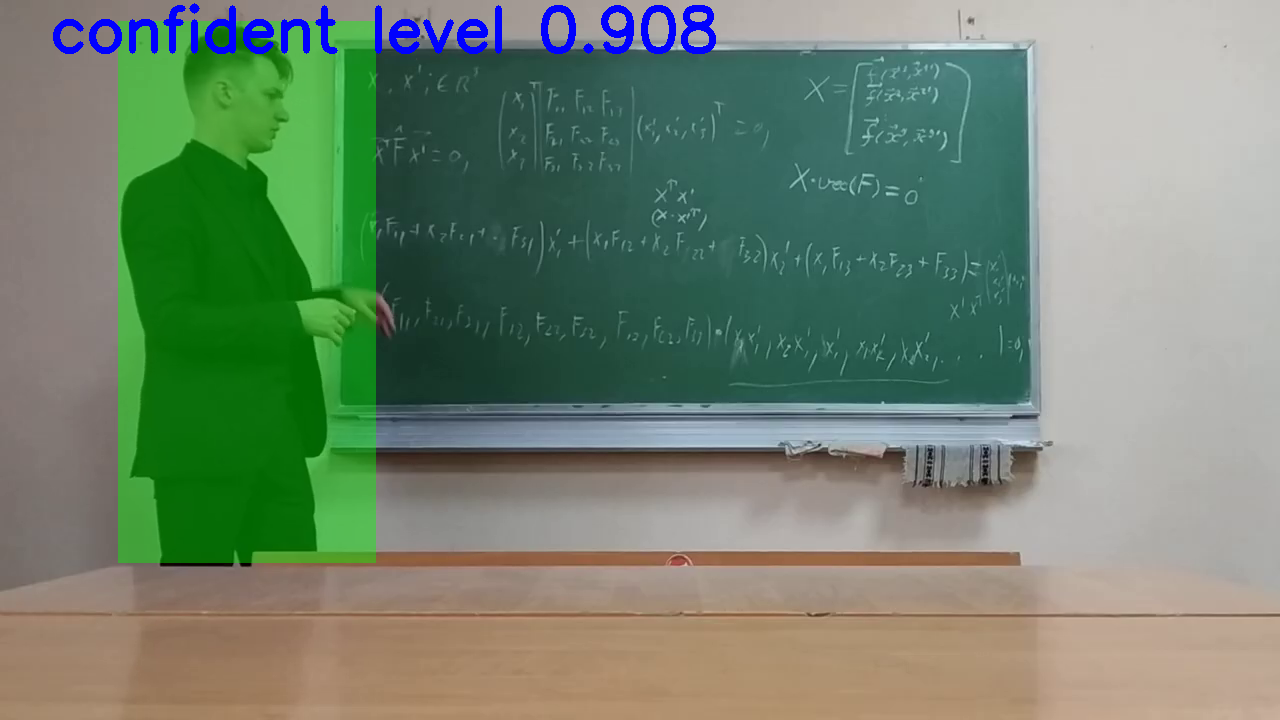
\includegraphics[width=0.35\textwidth]{images/krygin_geometry_yolov5n_17300}
    }
    \subfloat[\cite{algebra_geometry}]{
        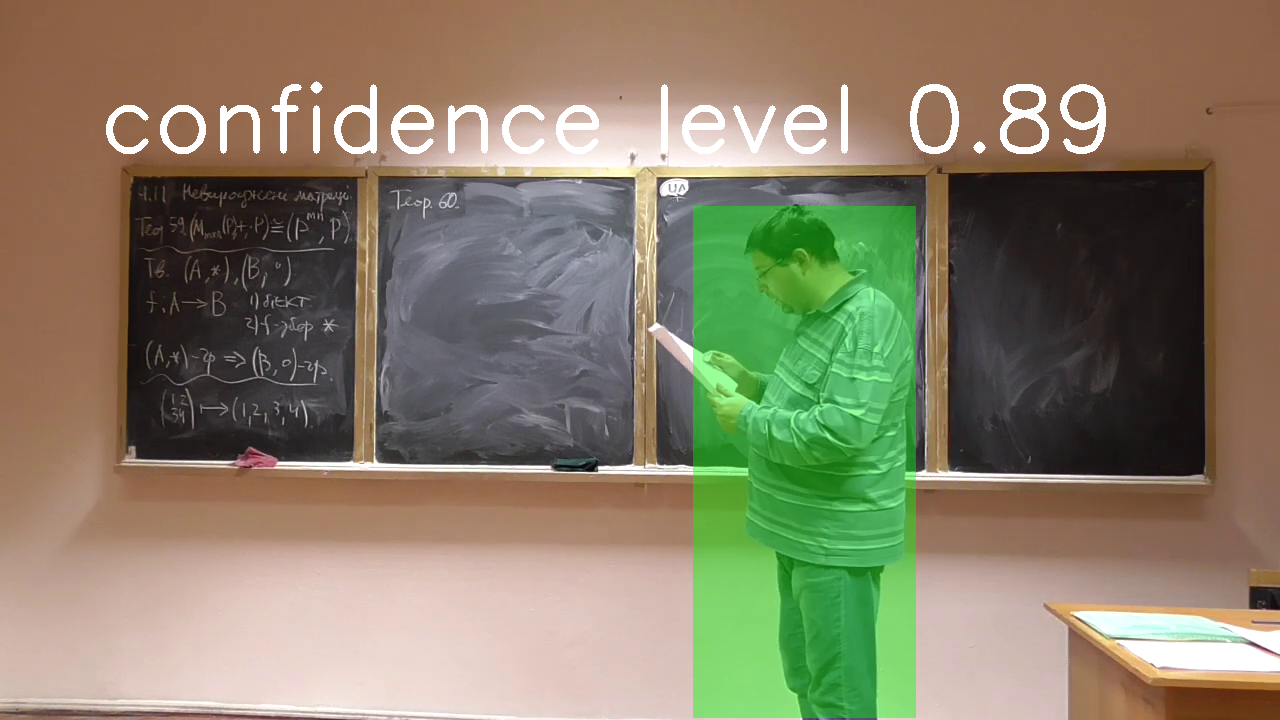
\includegraphics[width=0.35\textwidth]{images/algebra_geometry_yolov5n_9650}
    } \\
    \subfloat[\cite{yakovlev_numbers_theory_video}]{
        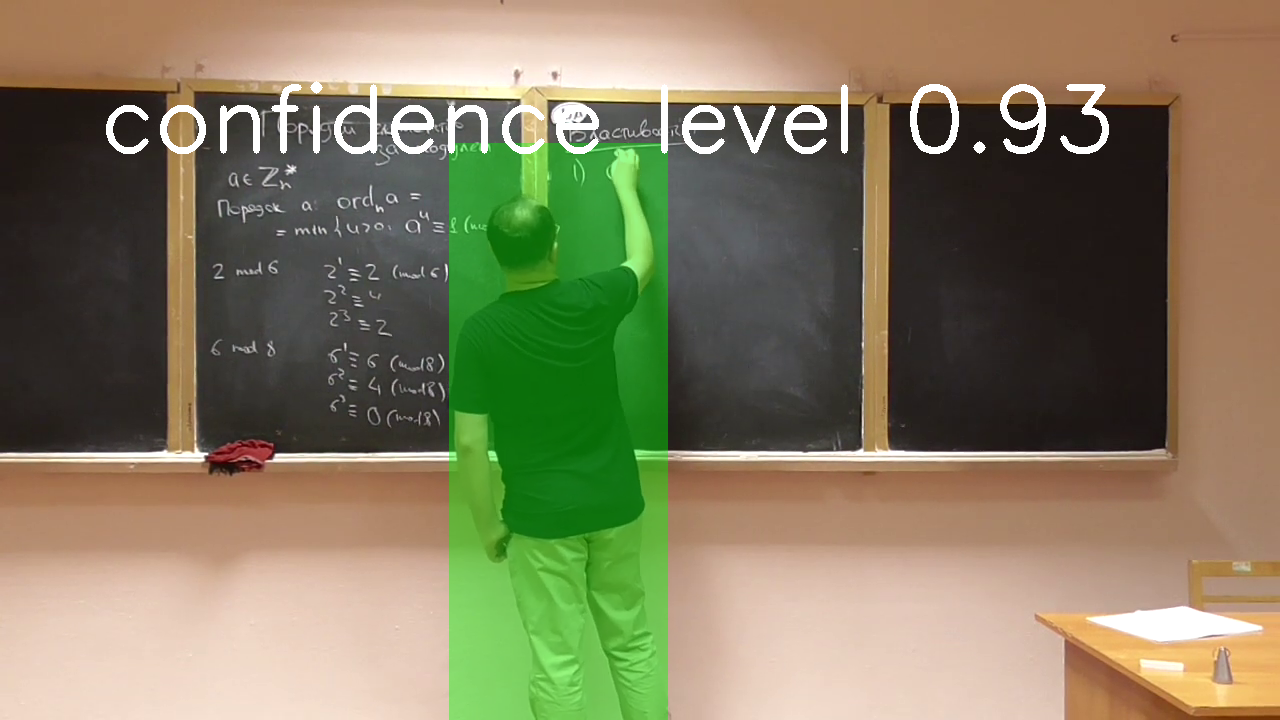
\includegraphics[width=0.35\textwidth]{images/yakovlev2_yolov5n_6500}
    }
    \subfloat[\cite{dorohovtsev_wiener_video}]{
        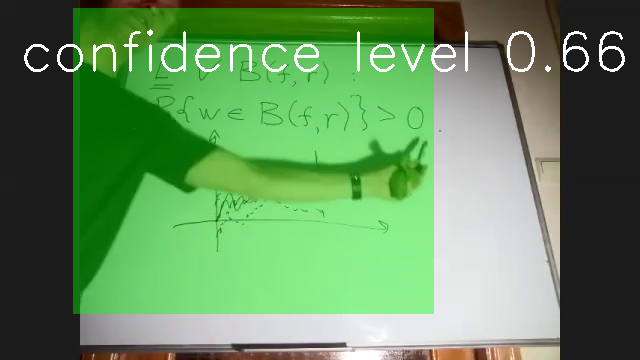
\includegraphics[width=0.35\textwidth]{images/dorohovtsev2_yolov5n_10650}
    }
    \caption{Приклад роботи yolov5n
        \label{fig:yolov5n_examples}
    }
\end{figure}

\begin{figure}[H]
    \centering
    \subfloat[\cite{krygin_geometry}]{
        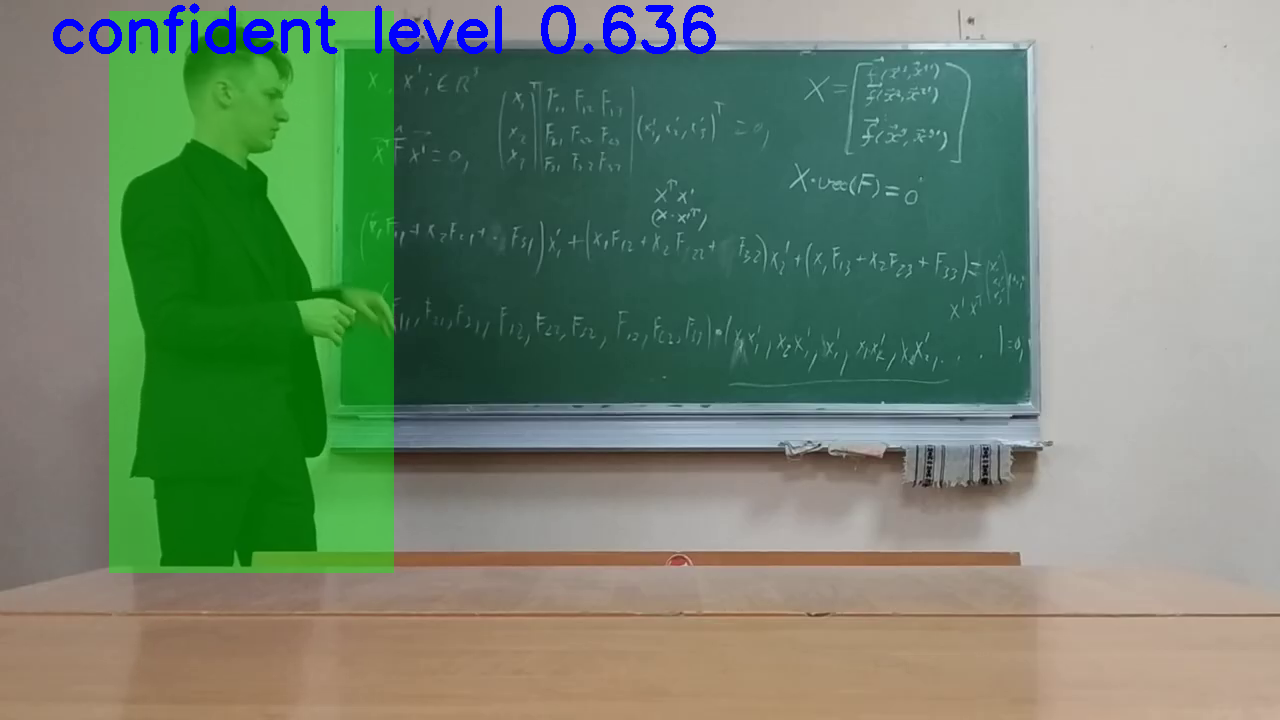
\includegraphics[width=0.35\textwidth]{images/krygin_geometry_ssdlite320_mobilenet_v3_17300}
    }
    \subfloat[\cite{algebra_geometry}]{
        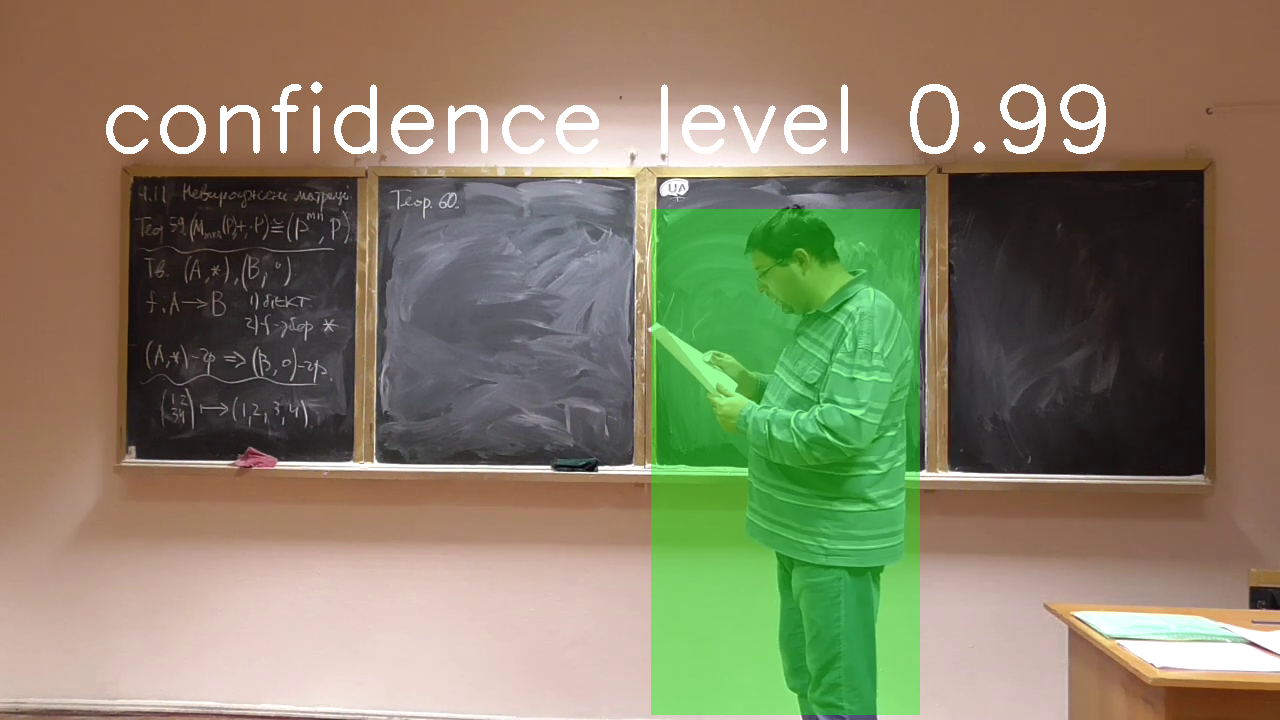
\includegraphics[width=0.35\textwidth]{images/algebra_geometry_ssdlite320_mobilenet_v3_9650}
    } \\
    \subfloat[\cite{yakovlev_numbers_theory_video}]{
        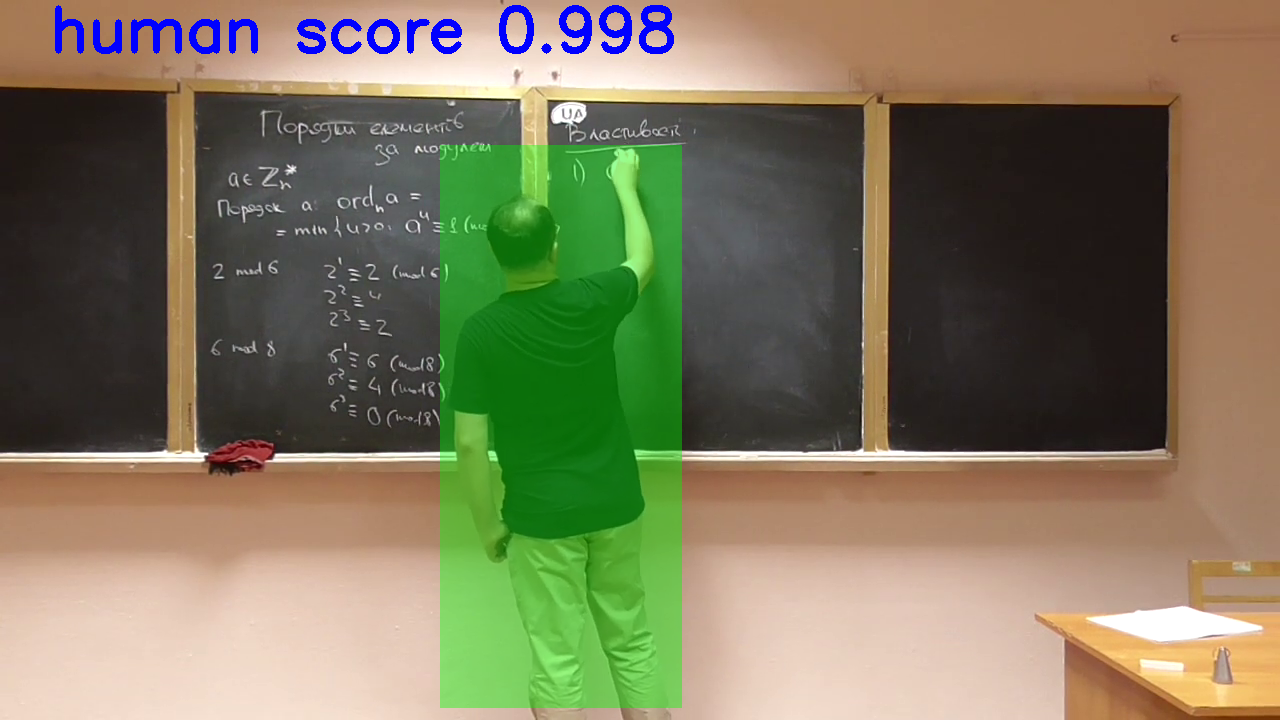
\includegraphics[width=0.35\textwidth]{images/yakovlev2_ssdlite320_mobilenet_v3_6500}
    }
    \subfloat[\cite{dorohovtsev_wiener_video}]{
        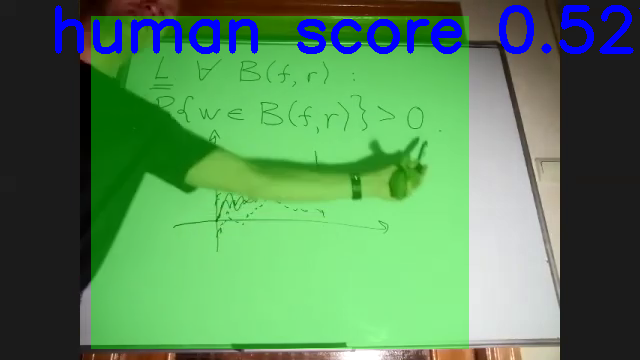
\includegraphics[width=0.35\textwidth]{images/dorohovtsev2_ssdlite320_mobilenet_v3_10650}
    }
    \caption{Приклад роботи ssdlite320-mobilenet-v3
        \label{fig:ssdlite320_mobilenet-v3_examples}
    }
\end{figure}

\begin{figure}[H]
    \centering
    \subfloat[\cite{krygin_geometry}]{
        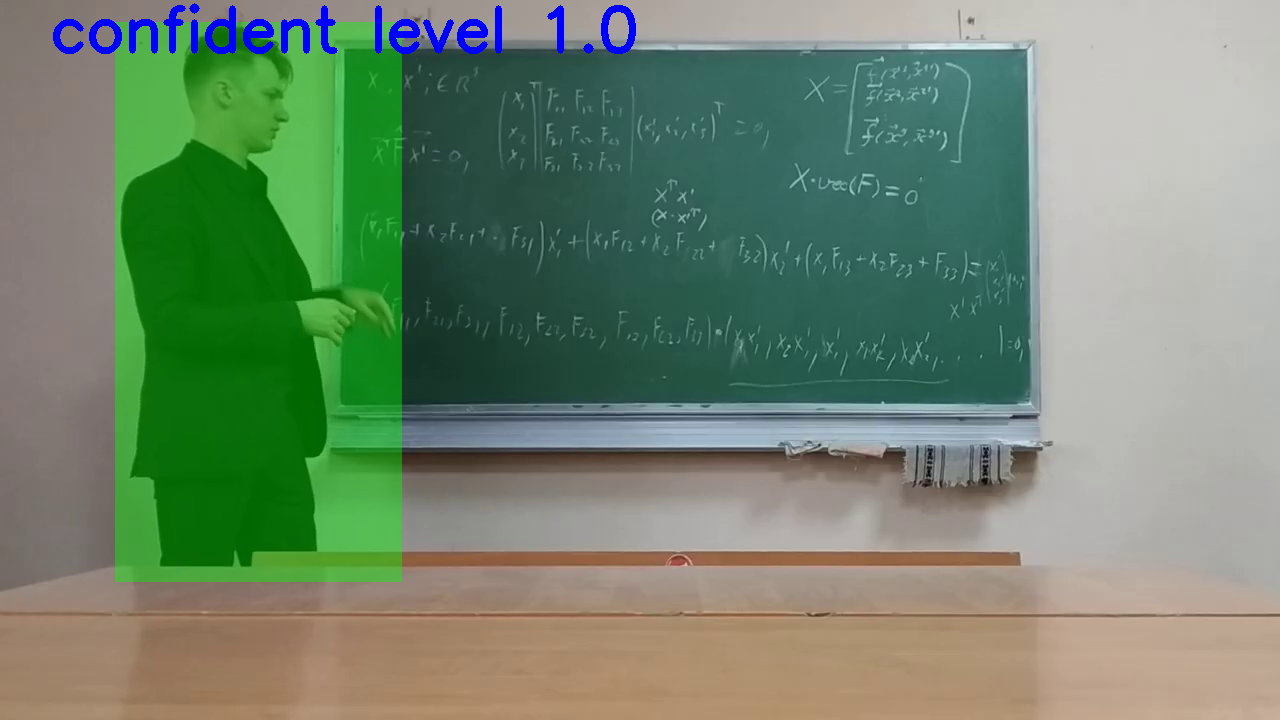
\includegraphics[width=0.35\textwidth]{images/krygin_geometry_fasterrcnn_mobilenet_v3_17300}
    }
    \subfloat[\cite{algebra_geometry}]{
        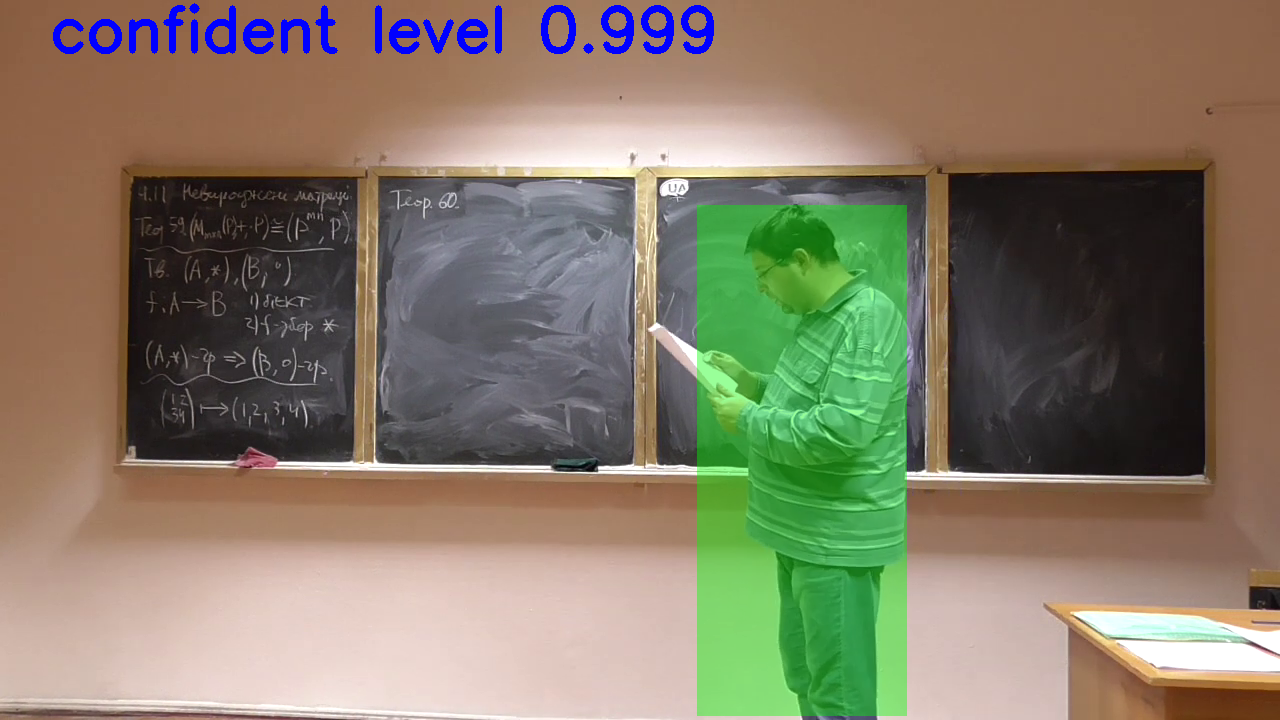
\includegraphics[width=0.35\textwidth]{images/algebra_geometry_fasterrcnn_mobilenet_v3_9650}
    }\\
    \subfloat[\cite{yakovlev_numbers_theory_video}]{
        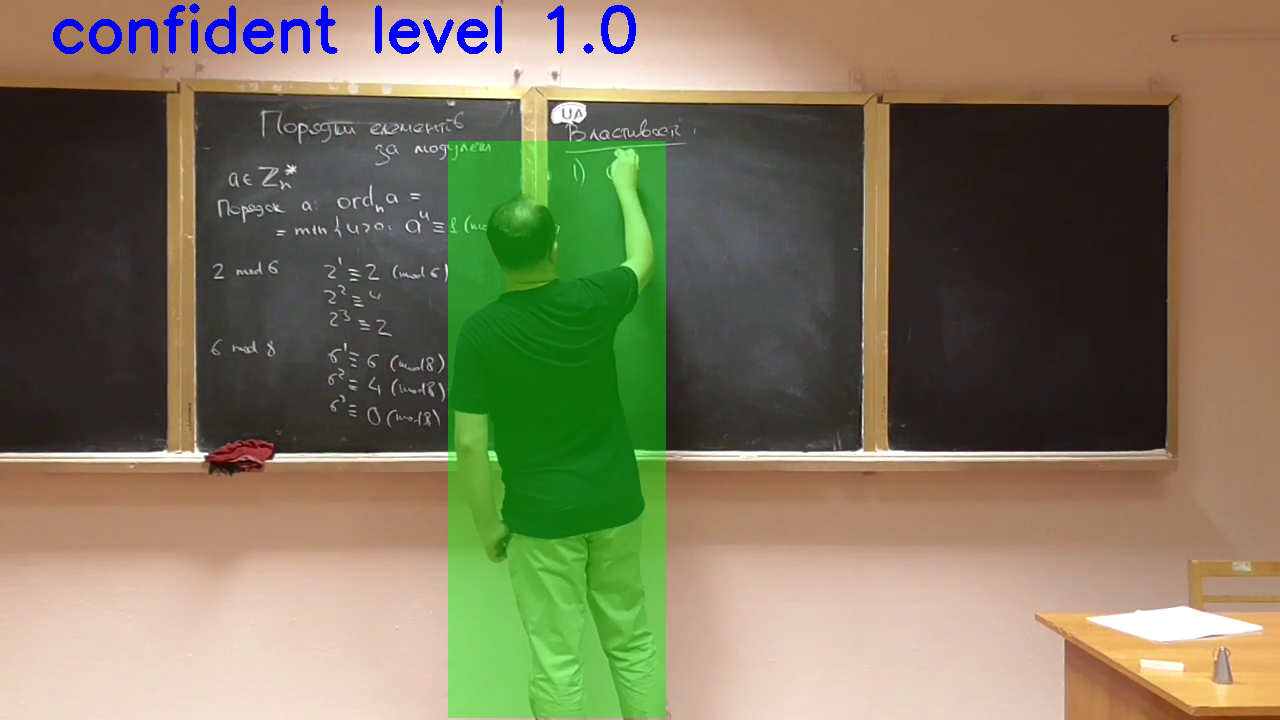
\includegraphics[width=0.35\textwidth]{images/yakovlev2_fasterrcnn_mobilenet_v3_6500}
    }
    \subfloat[\cite{dorohovtsev_wiener_video}]{
        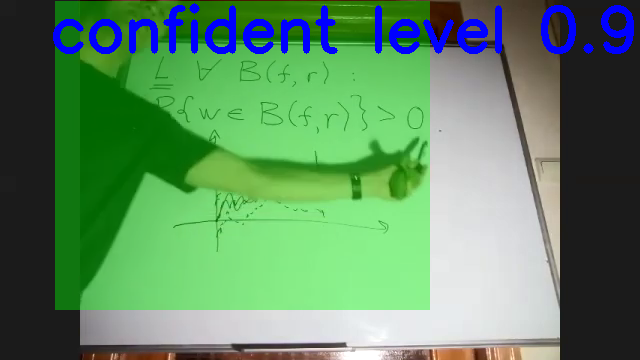
\includegraphics[width=0.35\textwidth]{images/dorohovtsev2_fasterrcnn_mobilenet_v3_10650}
    }
    \caption{Приклад роботи fasterrcnn-mobilenet-v3
        \label{fig:fasterrcnn_examples}
    }
\end{figure}

\section{Швидкість методів локалізації людини чи рухомих об'єктів}

Було протестовано 1000 разів отримання маски різними методами на картинці $720 \times 1280$ та
отриманий середній час обробки кадру (таб. \ref{tab:speed_methods_table}).
Варто відмітити, що картинка перед входом в шари згорток у згорткових нейромережах зменшується
до базового розміру для входу нейромережі. Така ж компресія робиться і для входу
в алгоритм Б-К, картинка зменшується удвічі.

\begin{table}[H]
    \begin{center}
        \caption{Таблиця швидкості згорткових нейромереж та алгоритму Б-К}
        \label{tab:speed_methods_table}
        \begin{tabular}{l|c|c|r}
            \textbf{yolov5n} & \textbf{ssdlite320-mobilenet-v3} & \textbf{fasterrcnn-mobilenet-v3} & \textbf{Boykov-Kolmogorov} \\
            \hline
            0.12             & 0.06                             & 0.12                             & 0.22                       \\
        \end{tabular}
    \end{center}
\end{table}


Як бачимо з табл. \ref{tab:speed_methods_table}, найшвидшим методом є ssdlite320-mobilenet-v3, а найдовшим є алгоритм Бойкова-Колмогорова.
Проте емпіричним шляхом було визначено, що кращі результати надає yolov5n.

\section{Результати створення панорами}


\section{Результати використання швидкої медіани}

На рис. \ref{fig:after_median_denoising} можна побачити як медіана справляється з шумом та артефактами компресії. Написи стали більш чіткими,
а фон дошки більш однорідним. Даний алгоритм доданий до інформаційної технології перетворення відео
з дошки у слайди.

\begin{figure}[H]
    \centering
    \subfloat[До]{
        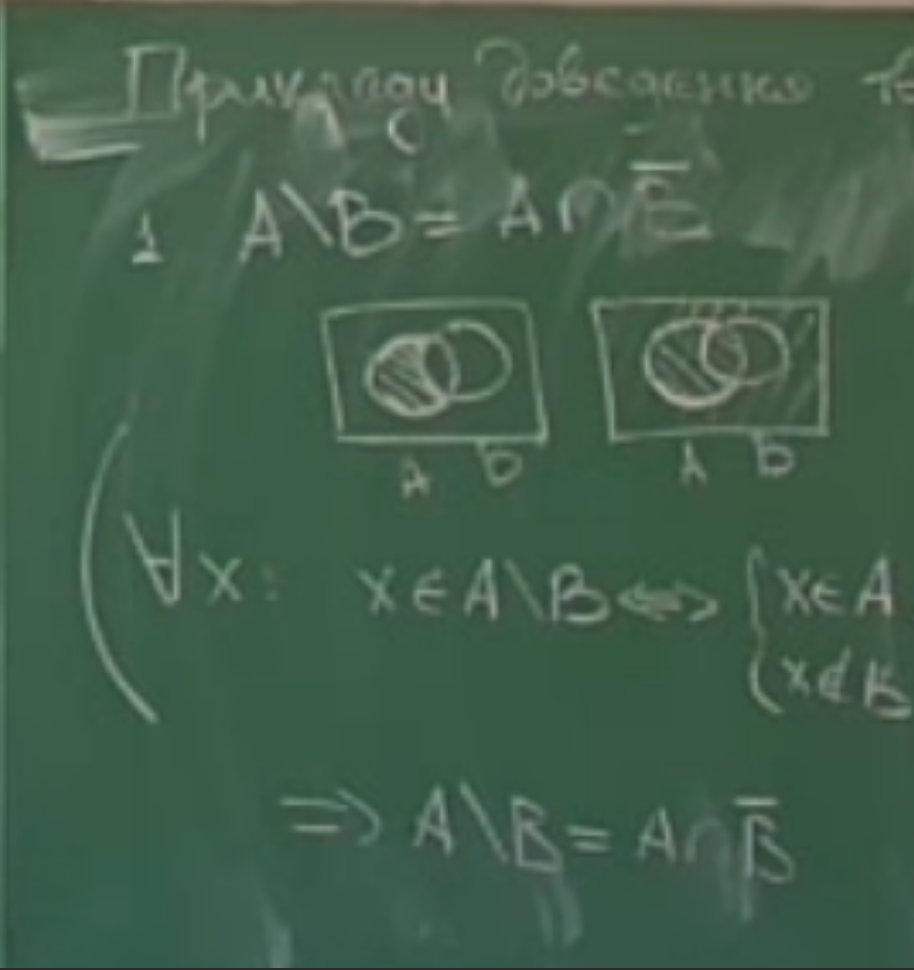
\includegraphics[width=0.35\textwidth]{images/frame_before_median}
    }
    \subfloat[Після]{
        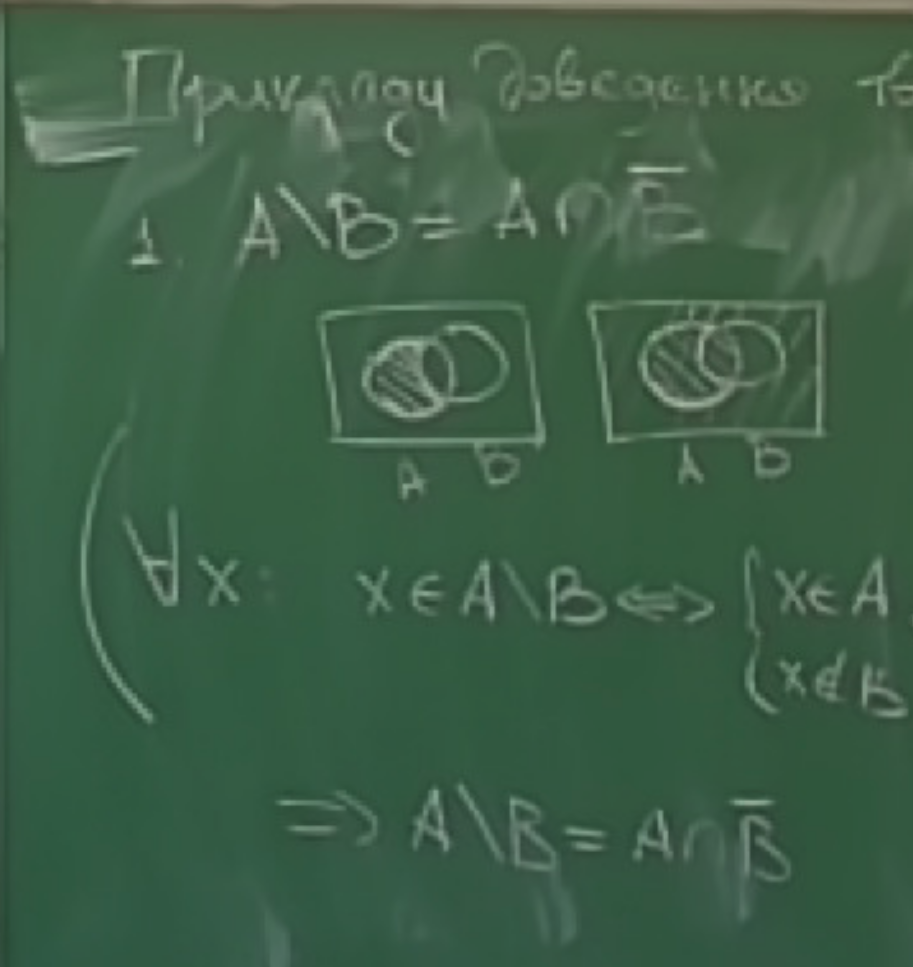
\includegraphics[width=0.35\textwidth]{images/frame_after_median}
        \label{fig:after_median_denoising}
    }
    \caption{Приклад роботи медіани для зображень \cite{yakovlev_discrete_math_video}
    }
\end{figure}
